\documentclass[aspectratio=169,11pt]{beamer}

\usetheme{Boadilla}
\usecolortheme{whale}
\usepackage{graphicx}
\usepackage{xcolor}
\usepackage{booktabs}

\definecolor{annblue}{RGB}{50,87,214}
\setbeamercolor{structure}{fg=annblue}
\setbeamertemplate{navigation symbols}{}
\setbeamertemplate{itemize items}[circle]

\title[ANNOT8]{ANNOT8}
\subtitle{Conversational PDF Annotation with Large Language Models}
\author{Paul Fishwick and Claude Code}
\date{\today}

\begin{document}

% ---- Slide 1: Title ----
\begin{frame}[plain]
  \titlepage
  \begin{center}
    \footnotesize\url{https://metaphorz.github.io/annot8/}
  \end{center}
\end{frame}

% ---- Slide 2: The Idea ----
\begin{frame}{The Idea}
  \begin{columns}[T]
    \begin{column}{0.54\textwidth}
      \begin{itemize}
        \item Technical PDFs --- patents, standards, reports --- are long
              and dense.
        \item Readers want to \textbf{ask questions} and keep the answers
              \textbf{attached to the source text}.
        \item \textbf{ANNOT8}: converse with an LLM about a PDF; every
              answer becomes an annotation on the passage it draws from.
        \item Motivated by a 304-page \emph{scanned} patent.
      \end{itemize}
    \end{column}
    \begin{column}{0.44\textwidth}
      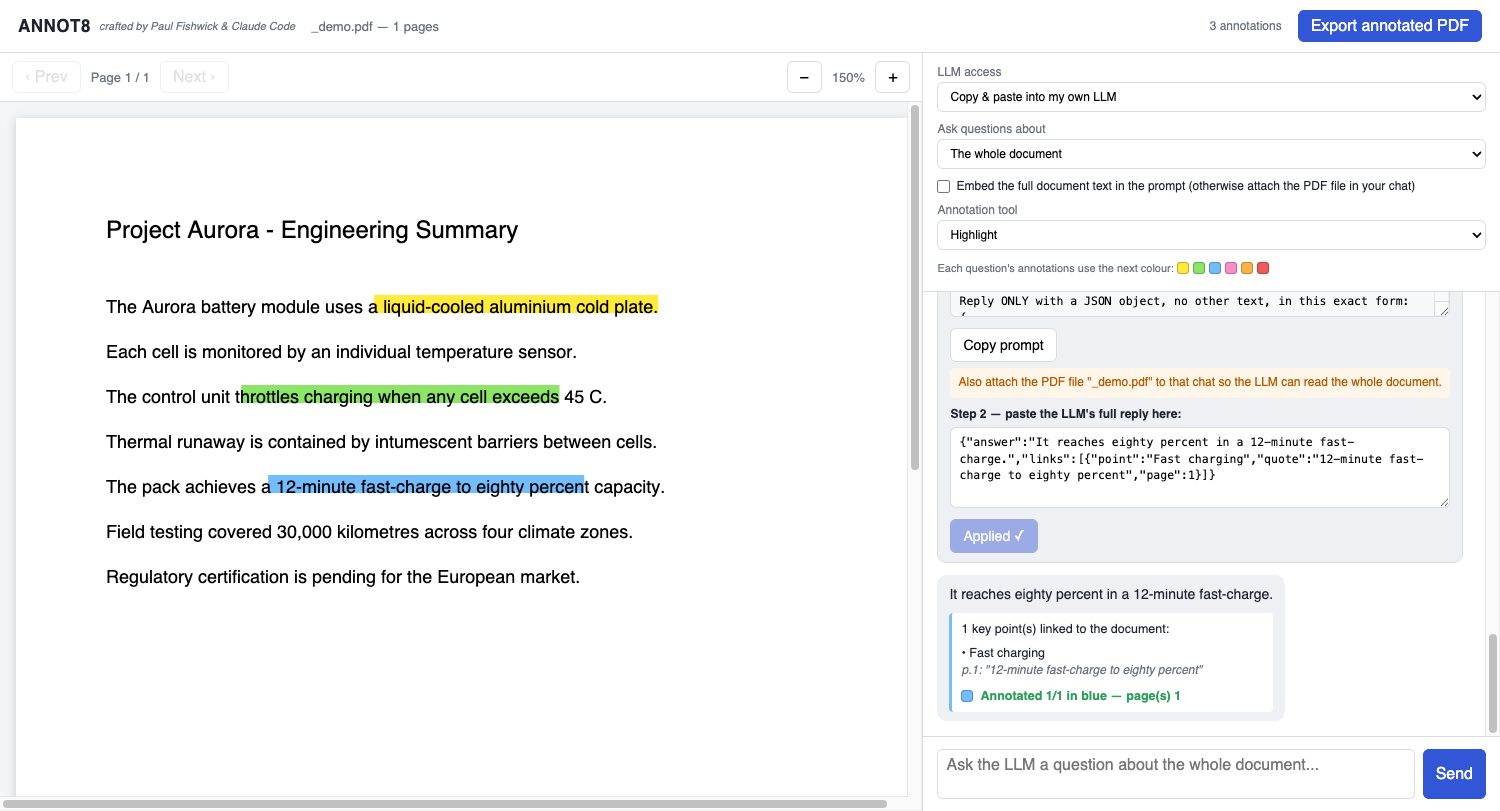
\includegraphics[width=\linewidth]{figures/fig_annotated.png}
      \vspace{2pt}
      \scriptsize\centering Answers auto-annotated, colour per question.
    \end{column}
  \end{columns}
\end{frame}

% ---- Slide 3: How It Works ----
\begin{frame}{How It Works}
  \begin{columns}[T]
    \begin{column}{0.52\textwidth}
      \begin{itemize}
        \item Drag-drop a PDF --- it stays in your browser.
        \item Ask about the \textbf{whole document} or the current page.
        \item Each answer is \textbf{auto-annotated}; the highlight colour
              cycles per question.
        \item Export a PDF with real Acrobat-style annotations.
      \end{itemize}
      \vspace{4pt}
      Two ways to reach an LLM:
      \begin{itemize}
        \item \textbf{Copy/paste} (default) --- use your own LLM.
        \item \textbf{OpenRouter API} --- latest Claude, GPT, Gemini.
      \end{itemize}
    \end{column}
    \begin{column}{0.46\textwidth}
      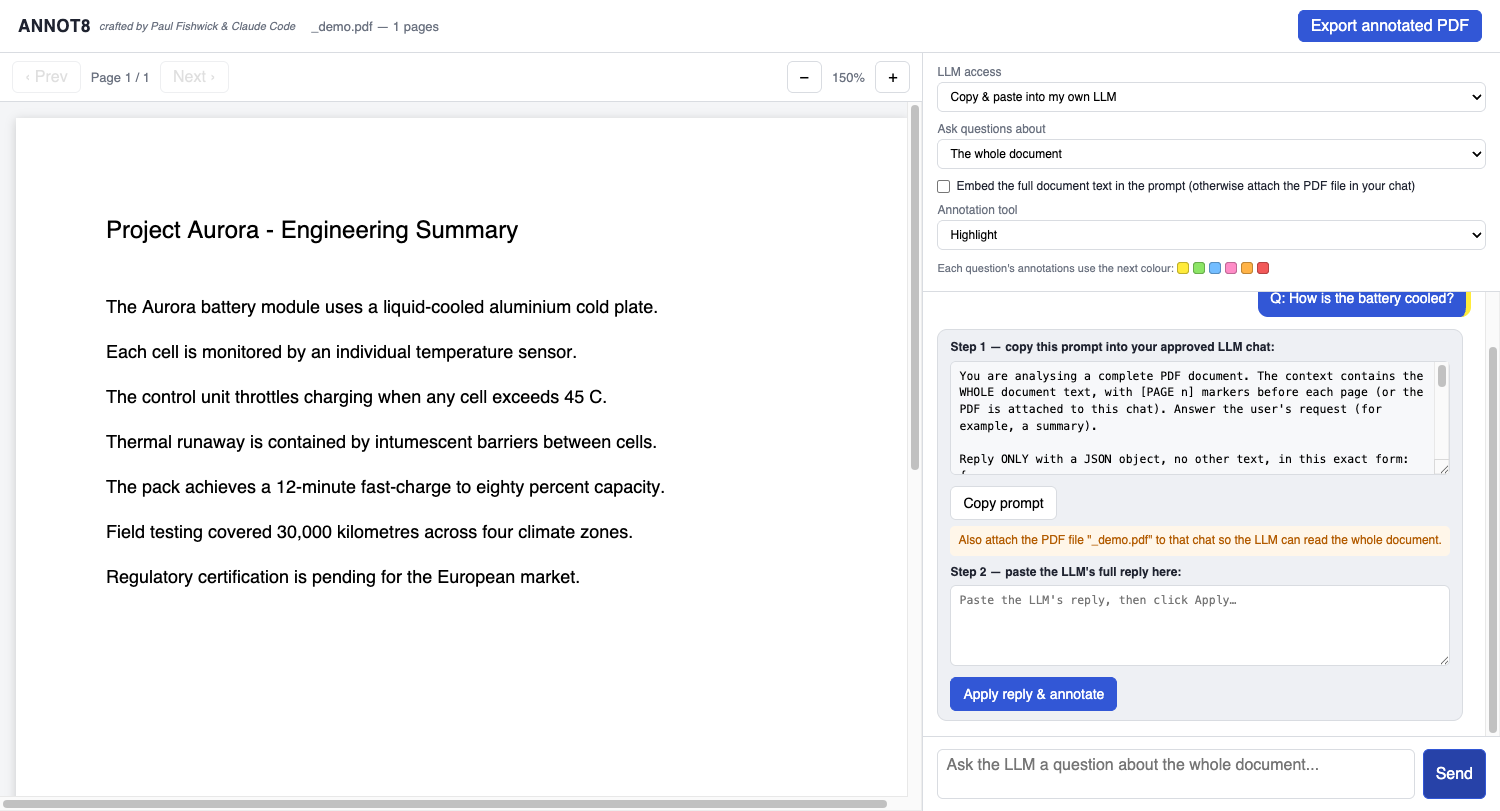
\includegraphics[width=\linewidth]{figures/fig_promptcard.png}
      \vspace{2pt}
      \scriptsize\centering Copy/paste mode: ANNOT8 builds the prompt;
      the reply is pasted back and applied locally.
    \end{column}
  \end{columns}
\end{frame}

% ---- Slide 4: Key Technology ----
\begin{frame}{Key Technology}
  \begin{itemize}
    \item \textbf{Text extraction} --- native PDF text layer per page, with
          Tesseract OCR fallback for scanned pages.
    \item \textbf{Fuzzy quote location} --- the hard part:
      \begin{itemize}
        \item The LLM's page numbers \emph{drift} --- off by 39--79 pages
              on the patent.
        \item OCR text is never copied verbatim.
        \item Content-token windowed matching searches \emph{every} page and
              trims the highlight to the densest cluster.
      \end{itemize}
    \item \textbf{Ten} Adobe Acrobat-style annotation tools; six colours.
    \item Two builds: a local Flask app, and a \textbf{100\% browser-only}
          build hosted on GitHub Pages.
  \end{itemize}
\end{frame}

% ---- Slide 5: Security ----
\begin{frame}{Security --- No Data Leak}
  For an enterprise user on a private, approved LLM, \textbf{nothing the
  user enters may leak.}
  \begin{itemize}
    \item Copy/paste mode: the prompt is shown for \emph{you} to copy ---
          ANNOT8 never transmits it.
    \item All libraries \emph{and} the Tesseract OCR engine are vendored ---
          works offline and behind corporate proxies.
    \item Self-hostable, so even page load never contacts GitHub.
  \end{itemize}
  \vspace{2pt}
  \begin{center}
  \small
  \begin{tabular}{lcc}
    \toprule
    \textbf{Session (network capture)} & \textbf{Requests} & \textbf{External} \\
    \midrule
    Copy/paste: load $\to$ annotate $\to$ export & 8 (own host) & none \\
    Scanned-PDF load + in-browser OCR & 10 (own host) & none \\
    \bottomrule
  \end{tabular}
  \end{center}
\end{frame}

% ---- Slide 6: Results & Links ----
\begin{frame}{Results}
  \begin{itemize}
    \item Automated tests: backend \textbf{29/29}, local UI \textbf{9/9},
          browser build \textbf{10/10} (Selenium).
    \item Whole-document summary of the 304-page patent: \textbf{5/5} key
          points located and highlighted, despite page drift up to 79 pages.
    \item Annotations export as real objects --- visible in Acrobat's
          Comments panel.
  \end{itemize}
  \vspace{6pt}
  \begin{block}{Try it / read more}
    \footnotesize
    App: \url{https://metaphorz.github.io/annot8/}\\
    Report: \url{https://metaphorz.github.io/annot8/report/annot8-report.pdf}\\
    Source: \url{https://github.com/metaphorz/annot8}
  \end{block}
  \vspace{4pt}
  \centering\small\textit{ANNOT8 --- crafted by Paul Fishwick and Claude Code.}
\end{frame}

\end{document}
